\begin{figure}[t]
\centering
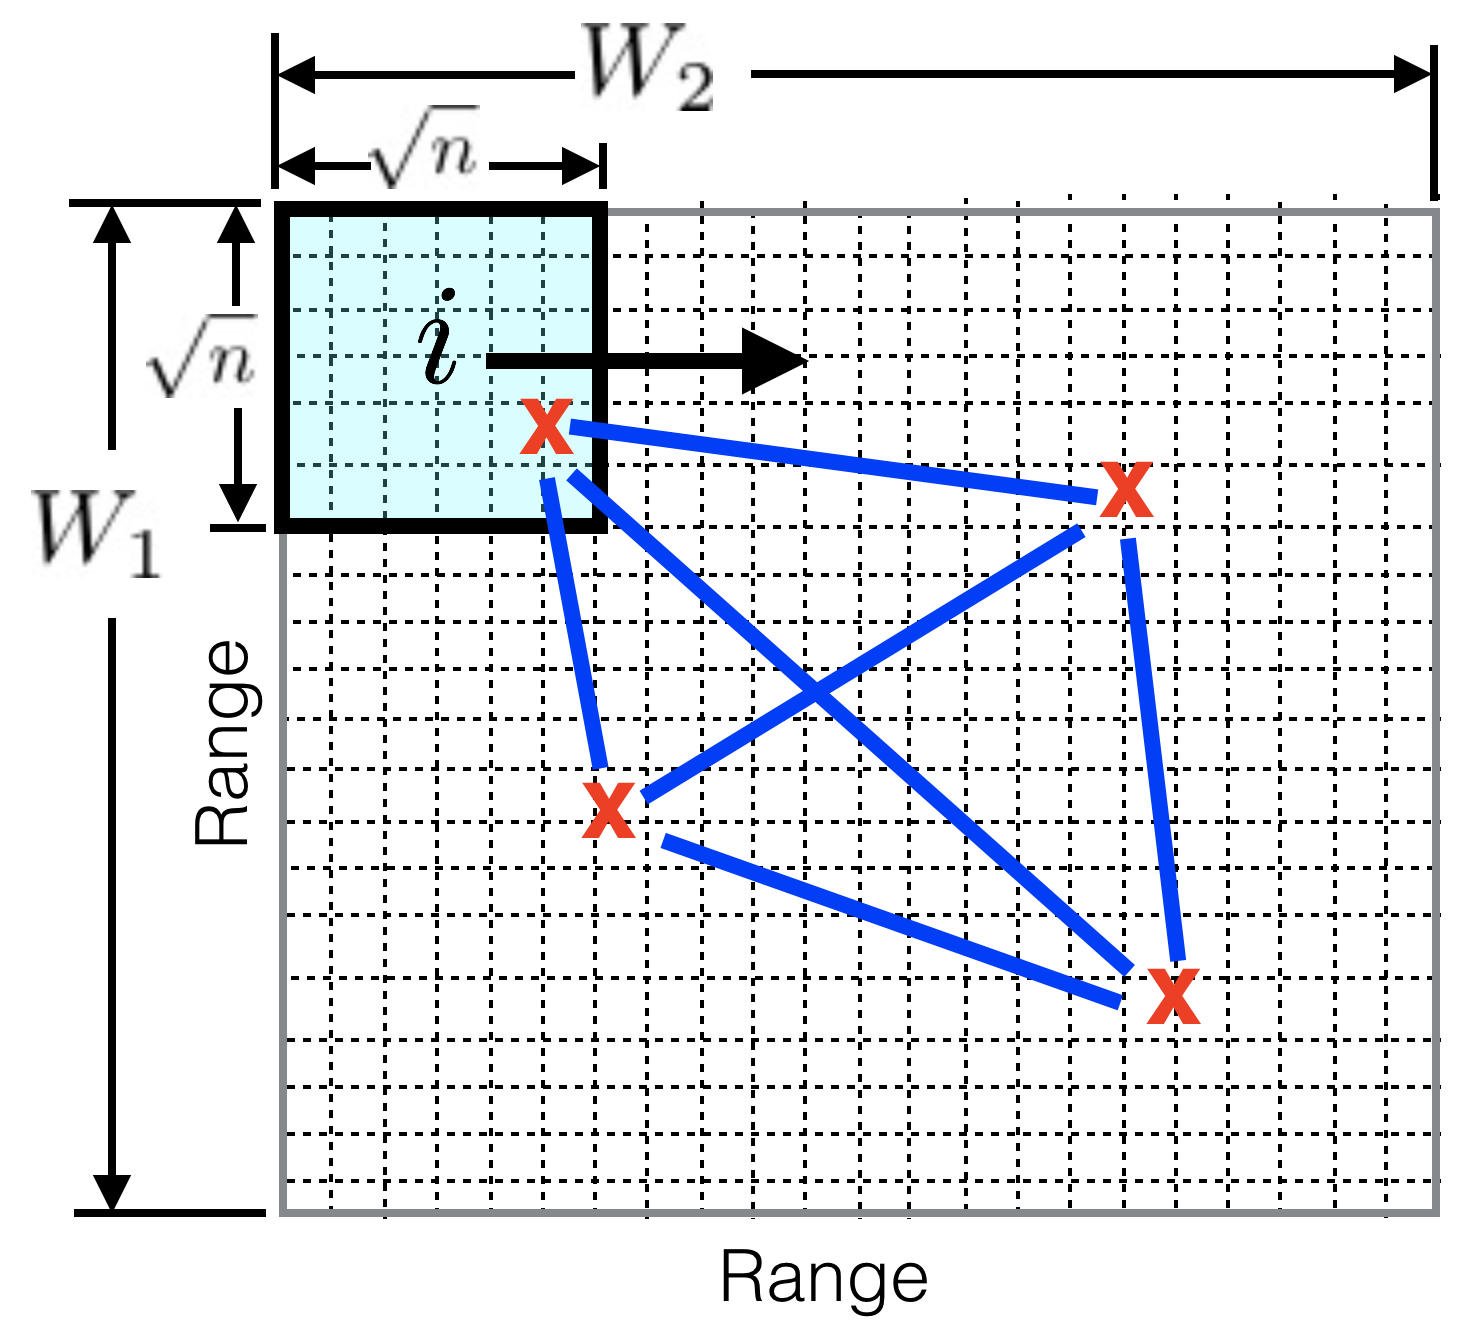
\includegraphics[width=6cm]{figs/patch.png} 
\caption{2D velocity image corresponds to  map divided into pixels (dashed boxes). The square image patch $i$ contains $n$ pixels. $W_1$ and $W_2$ are the vertical and horizontal dimensions of the image (in pixels), which give $I$ unique patches. Sensors are shown as red x's and the ray paths between the sensors are shown as blue lines.}
\label{fig:patchMap}
\end{figure}
\subsection{Tomography}
\yoav{I believe you are talking here about tomography, or reconstructing the environment. Can you write a paragraph of introduction, what is the problem? What is the desired solution?}
\rayan{I might be able to throw in some text about learning fast dictionaries, i.e., dictionaries learned from the data, but that also admit fast transforms like FFTs. Peter, Yoav, what do you think?}
{\bf Peter: Rayan, if it binds the proposal better together it would be excellent. We can always work on it anyway.}

After having observed and localized the sources we are here concerned with extracting the the environment $\bf E$. The environment is needed for any physical modeling and understanding of how the machine learning approaches work in practice. The models developed here could be aided by some know information about the environment $\bf E$, say the rooms in a house, or probability distributions of sound speed in the ocean or atmosphere.

We will have information about the travel-time and attenuation between a source and sensors. Or  travel-time and attenuation between sensors could be extracted by just observing noise\cite{shapiro2004, sabra2005, gerstoft2006}. In the initial setup, source and receivers locations are assumed known. 

We have worked on this problem for seismic modeling to develop separately two velocity models\cite{Bianco2018}, deemed the \textit{global} and \textit{local} models,  and briefly discuss dictionaries for sparse modeling. The global model considers the larger scale or global features and relates travel times to slowness. The local model considers smaller scale or more localized features with sparse modeling and is considered  to consist of sparse linear combinations of atoms from a dictionary
 We propose to use dictionary learning during the inversion to adapt dictionaries to specific slowness maps.

The global model has ben the basis of tomography and is repeated here for reference, slowness pixels (see Fig.~\ref{fig:patchMap}(a)) are represented by the vector $\mathbf{s'=s}_\mathrm{g}+\mathbf{s}_0\in\mathbb{R}^{N}$, where $\mathbf{s}_0$ is reference slownesses and $\mathbf{s}_\mathrm{g}$ is perturbations from the reference, here referred to as the {\it global slowness}, with $N=W_1W_2$. Similarly, the travel times of the $M$ rays are given as $\mathbf{t'=t+t}_0$, where $\mathbf{t}$ is the travel time perturbation and $\mathbf{t}_0$ is the reference travel time. The tomography matrix $\mathbf{A}\in\mathbb{R}^{M\times N}$ gives the discrete path lengths of $M$ straight-rays through $N$ pixels (see Fig.\ \ref{fig:patchMap}(a)). Thus  $\mathbf{t}$ and $\mathbf{s}_\mathrm{g}$ are related by the linear measurement model
%
%\begin{linenomath*}
\begin{equation}
\mathbf{t}=\mathbf{As}_\mathrm{g}+\epsilon,
\label{eq:linearTraveltime}
\end{equation}
%\end{linenomath*}
%
where $\mathbf{\epsilon}\in\mathbb{R}^M$ is Gaussian noise $\mathcal{N}(\mathbf{0},\sigma_\epsilon^2\bf{I})$, with mean $\mathbf{0}$ and covariance $\sigma_\epsilon^2\bf{I}$. We estimate the perturbations, with $\mathbf{s}_0$ and $\mathbf{t}_0=\mathbf{A}\mathbf{s}_0$ known. We call (\ref{eq:linearTraveltime}) the \textit{global model}, as it captures the large-scale features that span the discrete map and generates $\mathbf{t}$. 

Extracting of the local features is obtained via sparse modeling and dictionary learning.
Sparse modeling assumes that signals can be reconstructed using a few (sparse) vectors, called atoms, from a potentially large set of atoms, called a dictionary. Recent ocean acoustics works utilizing sparse modeling is beamforming\cite{Xenaki2014}, matched field processing \cite{Gemba2017}, and geoacoustic inversion \cite{gerstoft2018}. One challenge in sparse modeling is finding the best dictionary for sparsely representing specific signals. Such dictionaries can be composed of wavelets, or the discrete cosine transform (DCT). These predefined dictionaries perform well for many signals. However, using a form of unsupervised machine learning, called dictionary learning, optimal dictionaries can be learned directly from specific data\cite{mallat1999}. It has been shown that learned dictionaries outperform generic dictionaries when sufficient signal examples are available. Machine learning, and specifically dictionary learning, have recently obtained compelling results in ocean acoustics \cite{Bianco2017} and seismology\cite{kong2018}. 

%\yoav{I don't understand the following three paragraphs, can you give some technical details? Formulas?}
%In current work, we have developed a machine learning-based travel time tomography method called locally sparse travel time tomography (LST)\cite{bianco2018}. In LST, small scale local features contained in small rectangular groups of pixels, called patches, in an overall slowness (inverse  speed) map are constrained using a sparse model. Further, the sparsifying dictionary is adapted to the specific slowness data using dictionary learning. Larger scale, or global features spanning the  map, are constrained with least-squares regularization. Unlike conventional tomography, in which model features are forced to be exclusively smooth or discontinuous, the LST approach permits smooth and discontinuous local features via dictionary learning. 


Whereas many machine learning techniques in geoscience\cite{kong2018}, are reliant on large amounts of training data, LST\cite{bianco2018} requires none. In LST we adopt the adaptive dictionary learning paradigm from image denoising \cite{elad2010} and medical imaging\cite{ravishankar2011}, in which dictionaries are learned directly from patches of the corrupted image, obtained in \eqref{eq:linearTraveltime}. In LST, slowness dictionaries are learned from patches of a least squares regularized inversion, and are then used to reconstruct a sparsity-constrained slowness image. Assuming sufficiently dense ray sampling, the dictionary is initially unknown and is learned in parallel with the inversion. LST\cite{bianco2018} obtains high resolution by assuming that small patches of discrete slowness maps are repetitions of few elemental patterns from a dictionary of patterns, that is dictionary learning. 

Assuming that the travel paths between sensors has been estimated\cite{sabra2005,gerstoft2006} We propose the future development of machine learning-based tomography methods in acoustics. Such methods will help to more fully-exploit both existing environmental data $\bf E$, as well as very dense sampling from future arrays with many sensors. Such large scale, mobile, and deformable arrays, will use ambient noise processing \cite{sabra2005}, to obtain very dense and rich data sets. We propose  to: \\
(1) further develop a dictionary learning-based travel time tomography \cite{bianco2018}, accounting for uncertainty in the measurements and physics; \\
(2) formulate the dictionary learning-based approach as CNN via CSC; \\
(3) apply this CSC tomography framework to  data assimilation, to obtain higher-resolution estimates of the environment $\bf E$. \\

We further propose to develop  
(4) For EM signals, where the wave speed does not vary much the above formulation could be modified to do attenuation tomography.
(5) Acoustic event detection methods that leverage recent advances in machine learning.
(6) For unknown sensor location, only a graph of the sensor response is obtained. The edges of the graph will contain information related to travel time between nodes. It could here be useful to extract the information onto a manifold. From there further information could be extracted in the spatial dimension. A well-known example of this is that the location of cities in Switzerland could be constructed from the train schedule\cite{docmani2015}. With more sensors we would be able to extract both location and environmental information.  
%\end{itemize}

